\documentclass[12pt, english]{article}
\usepackage[utf8]{inputenc} %packages
\usepackage[T1]{fontenc}
\usepackage{babel}
\usepackage{listings}
\usepackage[text={20cm,25.5cm}]{geometry}
\looseness=-1
\usepackage[T1]{fontenc}
\usepackage{float}
\usepackage{graphicx}
\usepackage{caption}

\usepackage{hyperref} % For hyperlinks in the PDF
\usepackage{algpseudocode}
\usepackage{textcomp}
\usepackage{xcolor}
\usepackage{atbegshi}
\usepackage{csquotes}
\usepackage{algorithm}
\algdef{SE}{Begin}{End}{\textbf{begin}}{\textbf{end}}
\usepackage{etoolbox}
\usepackage{cite}
\usepackage{gensymb}
\usepackage{mathtools}
\DeclarePairedDelimiter{\ceil}{\lceil}{\rceil}
\usepackage{amsmath,amssymb,amsfonts}
\usepackage{multirow}
\usepackage{booktabs}
\usepackage{array}

\begin{document}
{\Large \textbf{Amit Sarker, Roll: 99}}\\

\par
Let \textit{N = (V, D, C)} be a constraint network. The constraint graph \textit{G = (V, E)} consists of \textit{V} vertices which is the variables of our constraint network and \textit{E} edges. There are some constraints \textit{c $\in$ C} enforced on these edges. I have used \textit{Arc consistency} algorithms for making the constraint network arc consistant.
\section{\textit{Design of the solution}}
\par
I have generated a random graph \textit{(graph = nx.erdos\_renyi\_graph(N, P))} using \textit{networkx} library, where \textit{N = number of nodes}, \textit{P = probability}, which means \textit{each edge is included in the graph with probability P independent from every other edge}. From the graph, I have generated the variables, domains and constraints list. \textit{Domains} are randomly selected with a fixed length domain size and I have used 10 \textit{constraints} which are assigned randomly to every node as I described my earlier problem description assignment. I have used this graph for all the arc-consistency algorithms and the comparisons and findings are described in the following sections.

\section{\textit{Comparisons}}
\par
I have compared all these four algorithms (\textbf{AC-1}, \textbf{AC-2}, \textbf{AC-3}, and \textbf{AC-4}) based on \textit{\textbf{total number of nodes vs run time}} and \textit{\textbf{probability of edges vs run time}}. For both cases, I have changed the domain size from \textit{10 to 100}, increased by \textit{30}. I have calculated the average run time for each domain size. I have taken an average of \textit{200 iterations} for both cases to calculate the average run time.\\\\
\hspace*{0.5cm}$\bullet$ \textit{\textbf{Total number of nodes vs Run time:}}
\begin{figure}[ht]
		{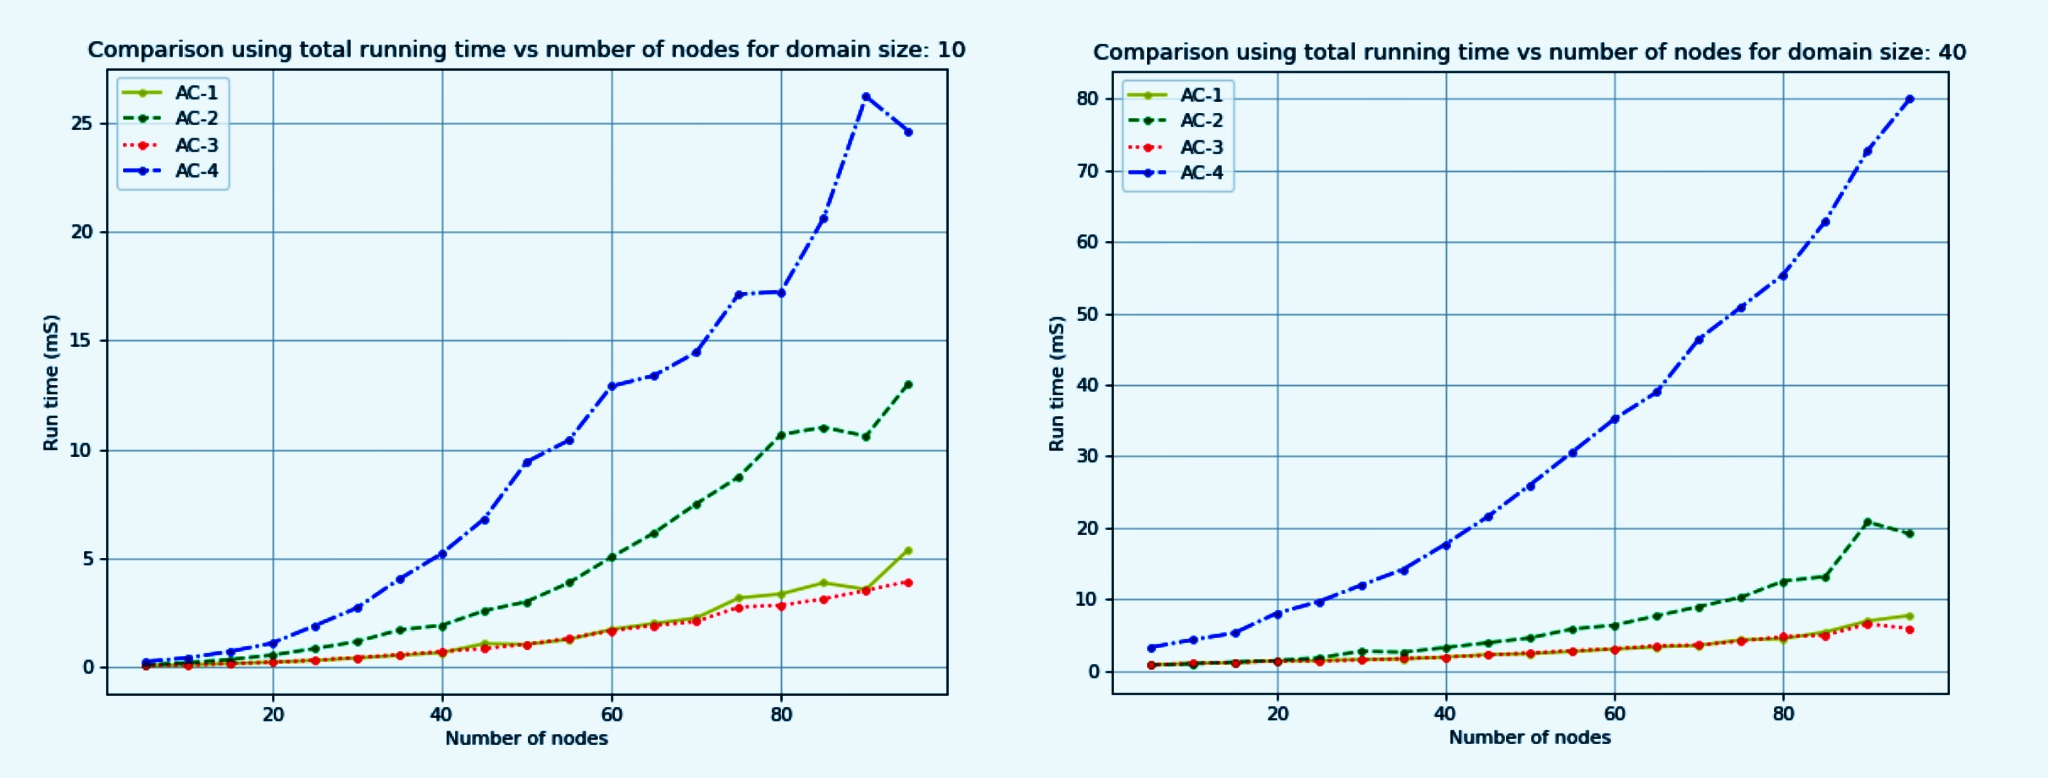
\includegraphics[width=\textwidth,height=2.6in]{1.jpeg}}
		{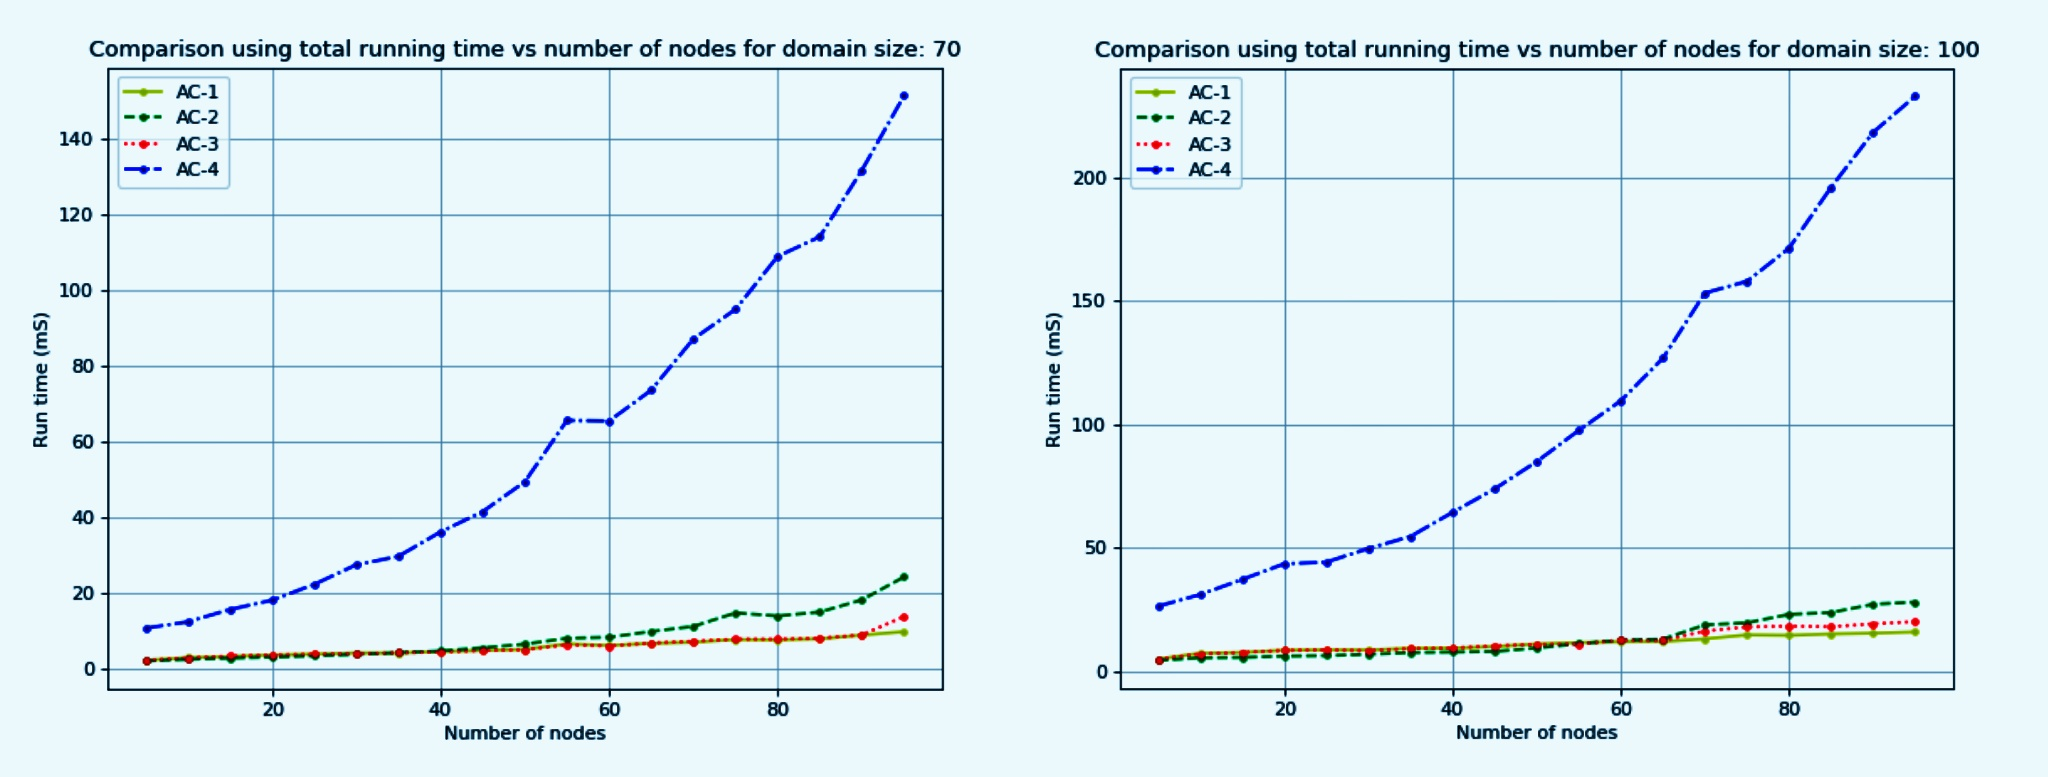
\includegraphics[width=\textwidth,height=2in]{2.jpeg}}
		\caption{\textbf{Total number of nodes vs Run-time for domain size 10, 40, 70, 100}}
        \label{fig: 1}
\end{figure}

\hspace*{0.5cm}$\bullet$ \textit{\textbf{Probability of edges vs Run time:}}
\begin{figure}[ht]
		{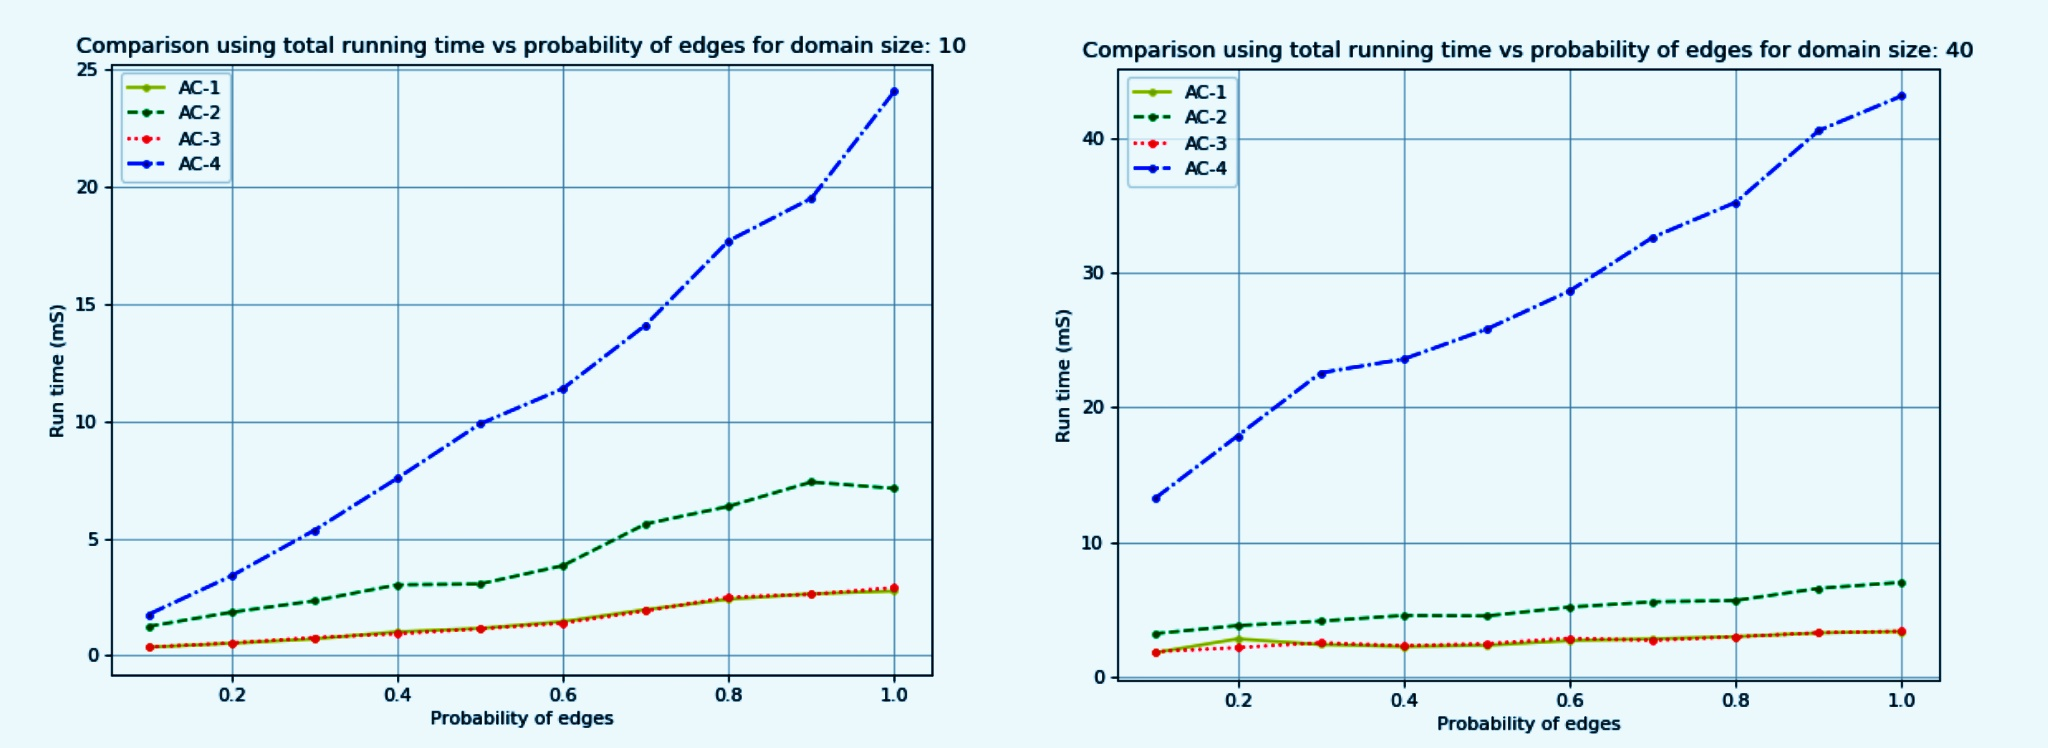
\includegraphics[width=\textwidth,height=2.6in]{3.jpeg}}
		{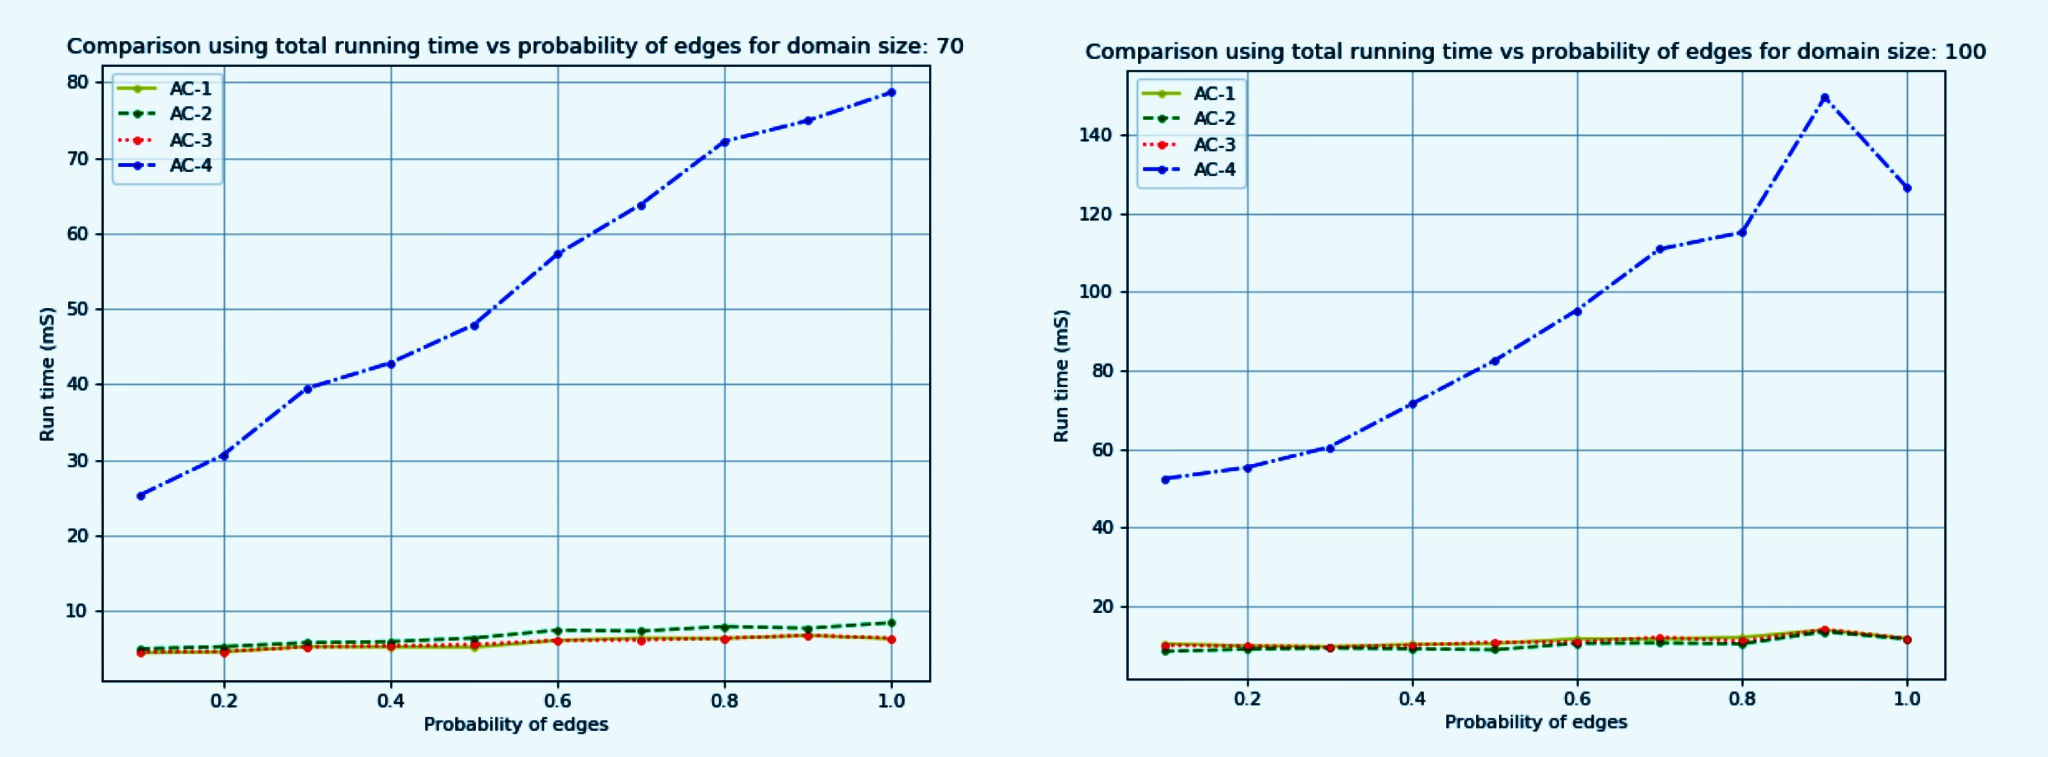
\includegraphics[width=\textwidth,height=2in]{4.jpeg}}
		\caption{\textbf{Probability of edges vs Run-time for domain size 10, 40, 70, 100}}
        \label{fig: 2}
\end{figure}

\par
For comparing the \textit{total number of nodes vs run time}, I have changed the value of the total number of nodes from \textit{5 to 95}, increased by \textit{5}. I have fixed the probability of edge to \textit{0.5} for this case. Figure~\ref{fig: 1} shows the comparison for \textit{total number of nodes vs run time}. For the second case, \textit{probability of edges vs run time}, I have changed the value of the probability of edge from \textit{0.1 to 1.0}, increased by \textit{0.1}. I have fixed the number of total nodes to \textit{50} for this case. Figure~\ref{fig: 2} shows the comparison for \textit{probability of edges vs run time}.



\section{\textit{Findings}}
\par
From the relative comparisons, it is clear that the performance of these four algorithms depends highly on \textit{domain size} as well as \textit{constraints selected}, \textit{number of nodes}, \textit{edges}, and other factors. From Figure~\ref{fig: 1}, we can say that, run time of \textit{AC-1} and \textit{AC-3} are close to one another. These two perform well in every case. This is because in the \textit{AC-3}, if the domain of a node has changed then I have checked the domain of each nodes adjacent with that particular node. In \textit{AC-1} algorithm when the domain of a node has changed I have checked every nodes for revise. But I have returned false if the domain of a single node becomes empty for all the four algorithms. For this reason, time complexity becomes O(e.k$^3$) for both cases and the run time of \textit{AC-1} and \textit{AC-3} are close in every case. For larger domain size, run time of \textit{AC-2} are also close to \textit{AC-1} and \textit{AC-3}. In \textit{AC-2} algorithm, we have made the graph consistent in an iterative increment process. First of all, we have made the graph consisting of less or equal \textit{j (j < total\_nodes)} nodes consistent. Then we have tried to make the graph consisting of less or equal \textit{j + 1, j + 2, ..., ..., i (i = total\_nodes)} nodes consistent. So, if domain size increases, time to perform a revise increases, but number of nodes are same. For this reason, \textit{AC-2} performs well in larger domain size. But \textit{AC-4} performs worst for all the cases. Time complexity of finding all the supports S[v$_j$, a$_j$] and counter(v$_i$, a$_i$, v$_j$) is \textit{O(n.k)} and \textit{O(e.k)} respectively, where \textit{n = number of nodes}, \textit{e = number of edges}, \textit{k = maximun length of a domain}. For these reasons, if the graph is already arc consistent or close to it, the best case time for \textit{AC-1} and \textit{AC-3} becomes \textit{O(e.k)}. But for \textit{AC-4} it is still \textit{O(e.k$^2$)}. That is why, \textit{AC-1} and \textit{AC-3} are outperforming \textit{AC-4} although \textit{AC-4} has the best run time in the worst case scenario. In Figure~\ref{fig: 2}, conditions are very similar to that of Figure~\ref{fig: 1}. Running time of \textit{AC-4} increases dramatically and \textit{AC-2} performs well for larger domains.



\section{\textit{Statistical significance Test}}
\par
I have performed the one-way \textit{ANOVA Tukey HSD Test} to determine whether there are any statistically significant differences between the mean running times of four arc consistency algorithms. Figure~\ref{fig: 3} shows that, all the possible pairs of arc consistency algorithm, the mean running times are significanty different except \textit{AC-1} vs \textit{AC-3}. This is quite expected, as we have seen from Figure~\ref{fig: 1} and Figure~\ref{fig: 2} that run time of \textit{AC-1} and \textit{AC-3} are very close to each other.

\begin{figure}[ht]
		{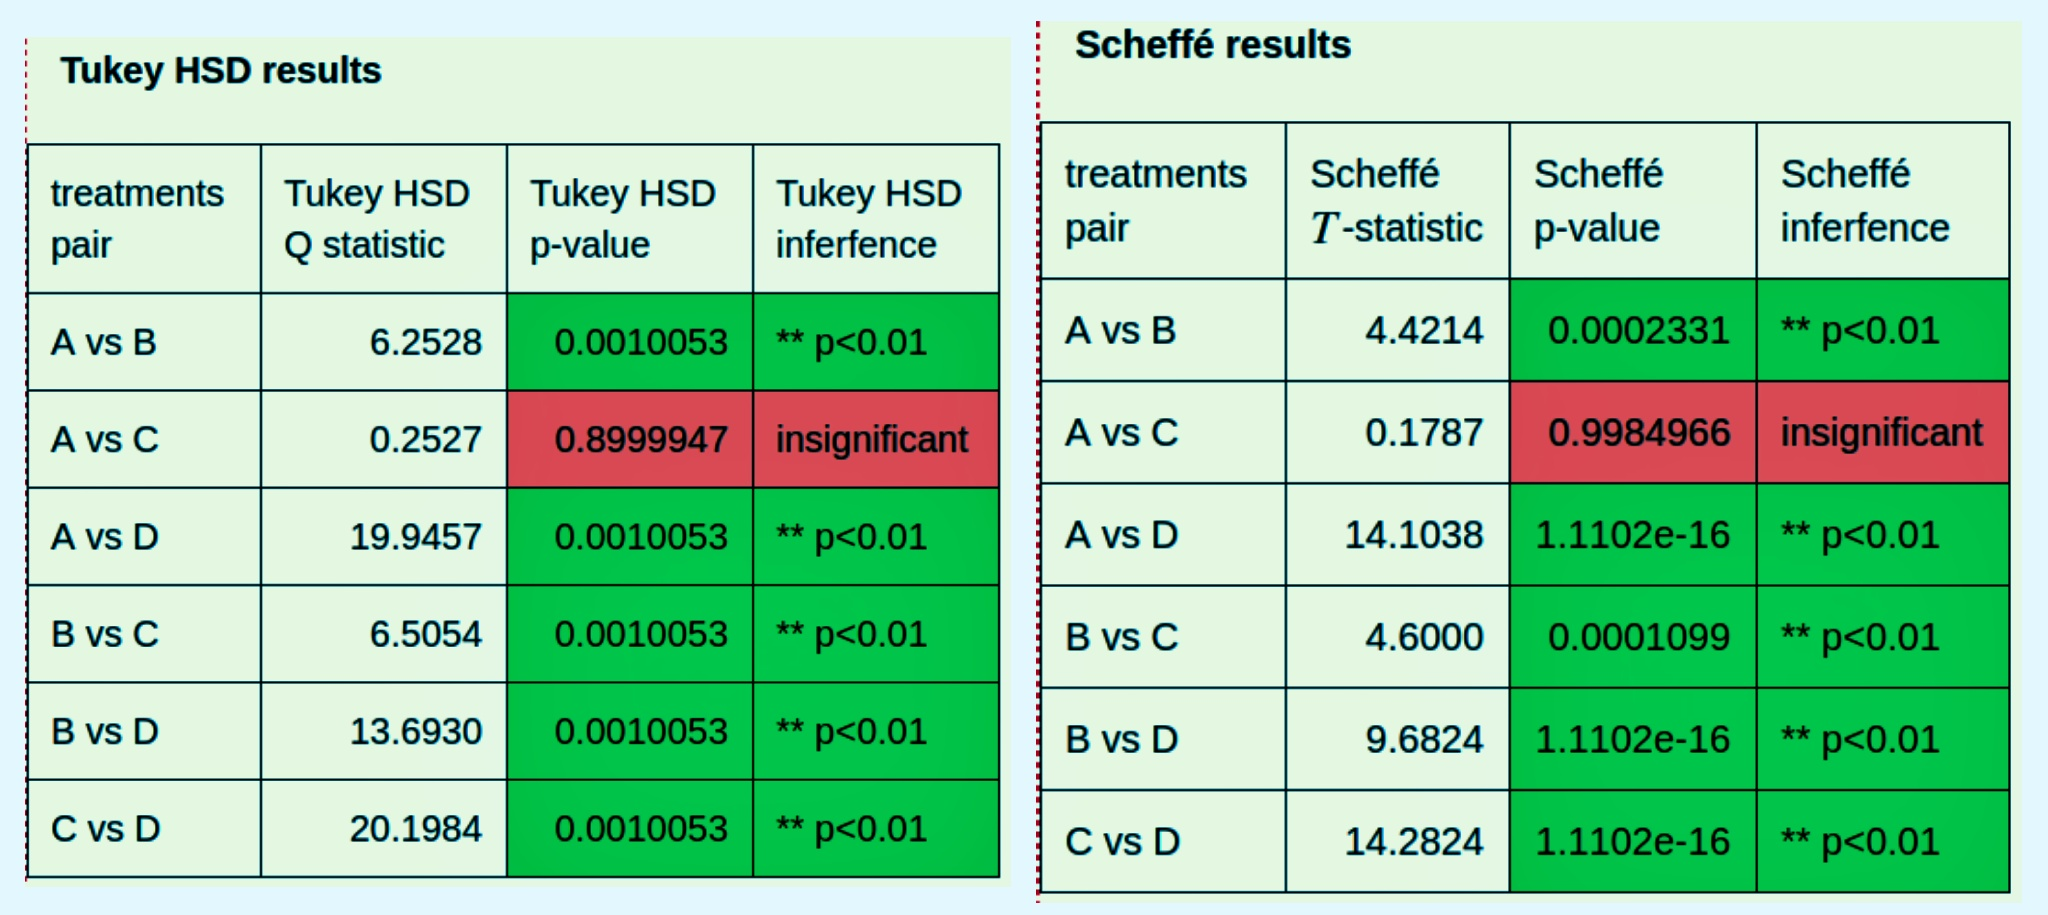
\includegraphics[width=\textwidth]{5.jpeg}}
		\caption{\textbf{One-way ANOVA with post-hoc Tukey HSD Test results}}
        \label{fig: 3}
\end{figure}


\end{document}
\grid